\scanpage{78}
\begin{center}
UNIVERSITE DES SCIENCES ET TECHNIQUES\\
DU LANGUEDOC\\
---\\
U.E.R. 5\\
Place Eugène Bataillon\\
34060 MONTPELLIER CEDEX\\
---
\end{center}
\begin{flushright}Montpellier, le\quad 12 février 1982\end{flushright}
\figure{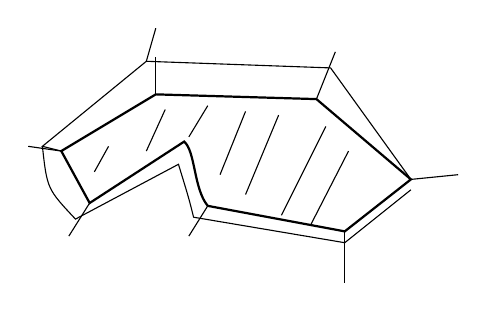
\begin{tikzpicture}[scale=1.2]
\draw[thick](0,.6)--(1,1.2)--(2.7,1.15)--(3.7,.3)--(3,-.25)--(1.55,.02)..controls(1.4,.2)and(1.42,.6)..(1.3,.7)--(.3,.05)--cycle;
\draw(0,.6)--(-.2,.65)--(.9,1.55)--(2.85,1.48)--(3.7,.3);\draw(-.2,.65)..controls(-.15,.2)..(.15,-.12)--(1.24,.46)..controls(1.35,.1)..(1.4,-.1)--(3,-.37)--(3.7,.19);
\foreach\a/\b/\c/\d in {.35/.38/.5/.65,.9/.6/1.1/1.04,1.35/.75/1.55/1.08,1.68/.35/1.95/1.02,1.95/.14/2.3/.98,2.33/-.08/2.8/.86,2.64/-.18/3.04/.6}{\draw[thin](\a,\b)--(\c,\d);}
\draw(-.35,.65)--(0,.6);\draw(.3,.05)--(.08,-.3);\draw(.9,1.55)--(1,1.9);\draw(1,1.2)--(1,1.6);\draw(2.7,1.15)--(2.9,1.65);\draw(3.7,.3)--(4.2,.35);\draw(3,-.25)--(3,-.8);\draw(1.55,.02)--(1.35,-.3);
\end{tikzpicture}}
\begin{center}\uline{D.E.A. DE MATHEMATIQUES}\end{center}
\begin{center}Organisation des cours pour l'année 1982 - 1983\end{center}
\figure{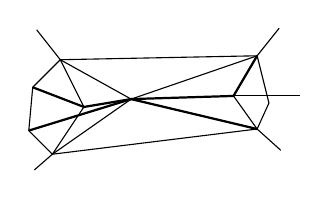
\begin{tikzpicture}
\draw(.1,.6)--(2.6,.65)--(2.75,.05)--(2.6,-.28)--(0,-.6)--(-.3,-.3)--(-.25,.25)--cycle;
\draw[thick](-.25,.25)--(.4,0)--(1,.1)--(2.3,.14)--(2.6,.65);\draw[thick](-.3,-.3)--(1,.1)--(2.6,-.28);\draw(.1,.6)--(1,.1)--(2.6,.65);\draw(0,-.6)--(1,.1)--(2.6,-.28);\draw(.1,.6)--(.4,0)--(0,-.6);\draw(2.6,.65)--(2.3,.14)--(2.6,-.28);\draw(.1,.6)--(-.2,.98);\draw(0,-.6)--(-.23,-.8);\draw(2.3,.14)--(3.15,.14);\draw(2.6,.65)--(2.88,1);\draw(2.6,-.28)--(2.9,-.55);
\end{tikzpicture}}
\begin{center}------\end{center}
\figure{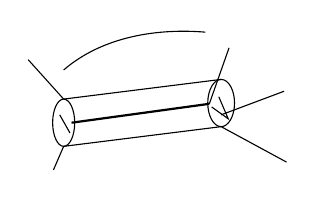
\begin{tikzpicture}
\draw(0,0)ellipse(.14 and .3);\draw(2,.25)ellipse(.17 and .3);\draw(0,.3)--(2,.55);\draw[thick](.1,0)--(1.85,.24);\draw(0,-.3)--(2,-.05);\draw(0,.3)--(-.45,.8);\draw(0,-.3)--(-.13,-.6);\draw(1.85,.24)--(2.1,.95);\draw(2,.1)--(2.8,.4);\draw(2,-.05)--(2.83,-.5);\draw(1.88,.2)--(2.09,.05)--(1.97,.33);\draw(-.05,.1)--(.08,-.13);\draw[thin](0,.67)..controls(.5,1.1)and(1.2,1.2)..(1.8,1.15);
\end{tikzpicture}}
Réunion le 26 février à 15 h, salle 208

\figure{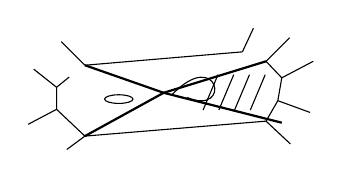
\begin{tikzpicture}
\draw(0,.45)--(2,.62);\draw(0,-.45)--(2.3,-.26);\draw[thick](0,.45)--(1,.1)--(2.5,-.28);\draw[thick](0,-.45)--(1,.1)--(2.3,.5);\draw(-.2,.3)--(-.36,.17)--(-.36,-.11)--(0,-.45);\draw(2.3,.5)--(2.5,.29)--(2.45,0)--(2.3,-.26);\draw(-.36,.17)--(-.65,.4);\draw(-.36,-.11)--(-.72,-.3);\draw(0,.45)--(-.3,.75);\draw(0,-.45)--(-.23,-.62);\draw(2.3,.5)--(2.6,.8);\draw(2.5,.29)--(2.9,.5);\draw(2.45,0)--(2.86,-.15);\draw(2.3,-.26)--(2.61,-.55);\draw(2,.62)--(2.14,.92);\draw(.43,.02)ellipse(.18 and .055);\draw[thin](1.1,.07)..controls(1.7,.7)and(1.87,-.2)..(1.3,.04);\foreach\x in {1.5,1.7,1.9,2.1}{\draw(\x,-.12)--(\x+.19,.33);}
\end{tikzpicture}}
Présence indispensable de tous les collègues intéressés par le fonctionnement du D.E.A. l'an prochain.

\figure{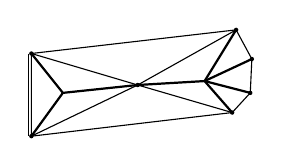
\begin{tikzpicture}
\draw(0,.45)--(2.6,.75)--(2.8,.38)--(2.78,-.05)--(2.55,-.3)--(0,-.6)--cycle;\draw[thick](0,.45)--(.4,-.05)--(1.35,.05)--(2.2,.1)--(2.6,.75);\draw[thick](0,-.6)--(.4,-.05);\draw[thick](2.2,.1)--(2.8,.38);\draw[thick](2.2,.1)--(2.78,-.05);\draw[thick](2.2,.1)--(2.55,-.3);\draw(0,.45)--(1.35,.05)--(2.55,-.3);\draw(0,-.6)--(1.35,.05)--(2.6,.75);\draw[xshift=-.04cm](0,.45)--(0,-.6);\foreach\x/\y in {0/.45,0/-.6,1.35/.05,2.6/.75,2.8/.38,2.78/-.05,2.55/-.3}{\fill(\x,\y)circle(.028);}
\end{tikzpicture}}
\begin{flushright}P. MOLINO\end{flushright}
\figure{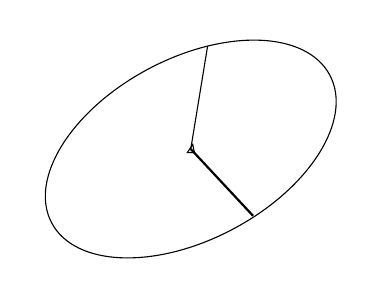
\begin{tikzpicture}[rotate=28]
\draw[thin](0,0)ellipse(2 and 1.15);\draw[thin](0,0)--(.8,1.05);\draw[thick](0,0)--(.3,-1.12);\draw(-.06,-.02)--(.05,.04)--(.02,-.06)--cycle;
\end{tikzpicture}}
\figure{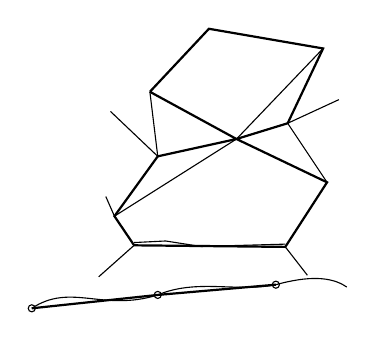
\begin{tikzpicture}
\draw[thick](0,1.4)--(.75,2.2)--(2.2,1.95)--(1.75,1)--(1.1,.8)--(.1,.58)--(-.45,-.18)--(-.2,-.55)--(1.72,-.57)--(2.25,.25)--(1.1,.8)--(0,1.4);
\draw(.1,.58)--(0,1.4);\draw(1.75,1)--(2.25,.25);\draw(-.45,-.18)--(1.1,.8)--(2.2,1.95);\draw(-.2,-.55)--(-.65,-.95);\draw(1.72,-.57)--(2,-.93);\draw(.1,.58)--(-.5,1.15);\draw(1.75,1)--(2.4,1.3);\draw(-.45,-.18)--(-.56,.07);\draw[yshift=.035cm](-.2,-.55)--(.2,-.53)--(.65,-.6)--(1.72,-.57);
\draw[thick](-1.5,-1.35)--(.1,-1.18)--(1.6,-1.05);\draw(-1.5,-1.35)..controls(-1,-1.02)and(-.6,-1.4)..(.1,-1.18)..controls(.6,-.97)and(1.1,-1.15)..(1.6,-1.05)..controls(2,-.94)and(2.3,-.94)..(2.5,-1.08);\foreach\x/\y in {-1.5/-1.35,.1/-1.18,1.6/-1.05}{\draw(\x,\y)circle(.045);}
\end{tikzpicture}}
\figure{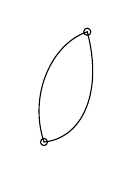
\begin{tikzpicture}
\draw(0,0)..controls(-.2,.6)and(.1,1.25)..(.55,1.4)..controls(.75,.65)and(.5,.05)..cycle;\draw(0,0)circle(.045);\draw(.55,1.4)circle(.045);
\end{tikzpicture}}
\figure{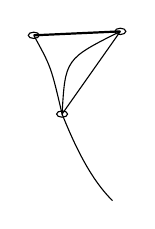
\begin{tikzpicture}
\draw[thick](0,1)--(1.1,1.05);\draw(0,1)..controls(.22,.6)..(.36,0)--(1.1,1.05);\draw[thin](.36,0)..controls(.4,.7)..(1.1,1.05);\draw(.36,0)..controls(.6,-.6)and(.8,-.9)..(1,-1.1);\foreach\x/\y in {0/1,1.1/1.05,.36/0}{\draw(\x,\y)ellipse(.07 and .04);}
\end{tikzpicture}}
\mspage{77}
